\setAuthor{Tundmatu autor}
\setRound{lahtine}
\setYear{2006}
\setNumber{G 4}
\setDifficulty{4}
\setTopic{Dünaamika}

\prob{Kivi}
Paelaga lae külge kinnitatud kivi liigub mööda horisontaaltasapinnas asuvat ringjoont, mille kaugus laest $h = \SI{1,25}{m}$. Leida kivi tiirlemisperiood $\tau$. 

\hint
Kivile mõjuva paela tõmbepinge $T$ ja raskusjõu $mg$ resultant on kesktõmbejõuks, mis on suunatud horisontaaltasapinnas sissepoole.

\solu
Kivile mõjuvaks kesktõmbejõuks on paela tõmbepinge $T$ projektsioon tiirlemise
tasapinnale $F = T \sin \varphi$ (vt joonist), kus $\varphi$ on nurk paela ja vertikaalsihi vahel. Newtoni teine seadus kivi liikumise jaoks mööda ringjoont raadiusega $R$ näeb välja:
\begin{equation} \label{2006-lahg-04:eq1}
m\omega^2R = T \sin \varphi,
\end{equation}
kus $\omega = 2\pi /\tau$ --- kivi nurkkiirus ja $m$ --- kivi mass. Kuna vertikaalsuunas kivil kiirendus puudub, järelikult kivile mõjuvate jõudude projektsioonid vertikaalteljele annavad summas nulli:
\begin{equation} \label{2006-lahg-04:eq2}
T \cos\varphi = mg.
\end{equation}
Jagades valemi (\ref{2006-lahg-04:eq1}) valemiga (\ref{2006-lahg-04:eq2}), saame
\[
\tan \varphi = \frac{\omega^2R}{g}.
\]
Arvestades, et $\tan \varphi = R/h$, saame
\[
\frac{\omega^{2} R}{g}=\frac{R}{h} \quad \Rightarrow \quad \omega=\sqrt{\frac{g}{h}},
\]
ehk
\[
\tau=\frac{2 \pi}{\omega}=2 \pi \sqrt{\frac{h}{g}}=2 \cdot \num{3,14} \cdot \sqrt{\frac{\num{1,25}}{\num{9,81}}} \approx \SI{2,24}{s}.
\]

\begin{center}
	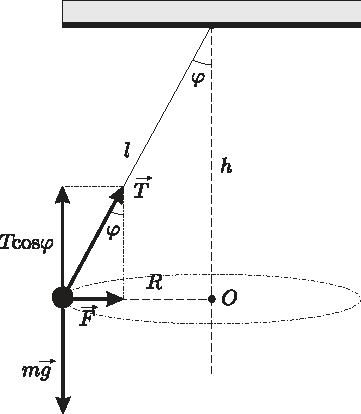
\includegraphics[width=0.7\linewidth]{2006-lahg-04-lah}
\end{center}
\probend